% -*- coding: utf-8 -*-
\documentclass[a4paper,12pt]{article}
\usepackage[T1]{fontenc}
\usepackage[utf8]{inputenc}
\usepackage[russian]{babel}
\usepackage{amsmath,amsfonts,amssymb}
\usepackage{graphicx}
\usepackage{booktabs}
\usepackage{caption}
\usepackage{float}            % для жёсткого размещения [H]
\usepackage{geometry}
\geometry{margin=2.5cm}

\title{Краткий отчёт о результатах экспериментов}
\author{~}
\date{}

\begin{document}
\maketitle

%--------------------------------------------------
\section*{1. Влияние параметров распределения (Часть\,1)}

\begin{figure}[H]
    \centering
    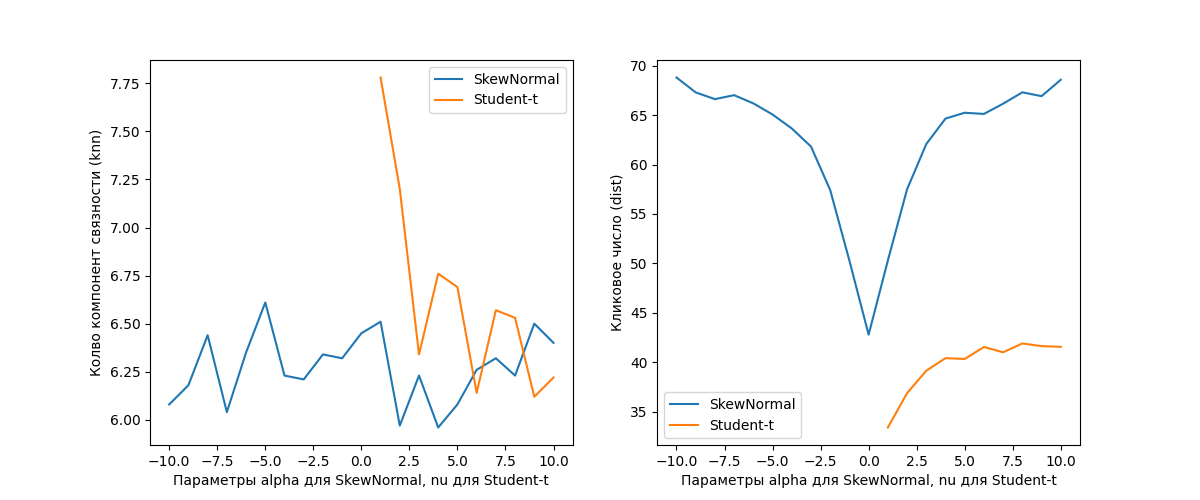
\includegraphics[width=0.95\textwidth]{Graphics/part1_results_Askar.png}
    \caption{Изменение графовых метрик при варьировании параметров SkewNormal/Student-$t$ (серия Аскара).}
    \label{fig:part1-askar}
\end{figure}

\begin{figure}[H]
    \centering
    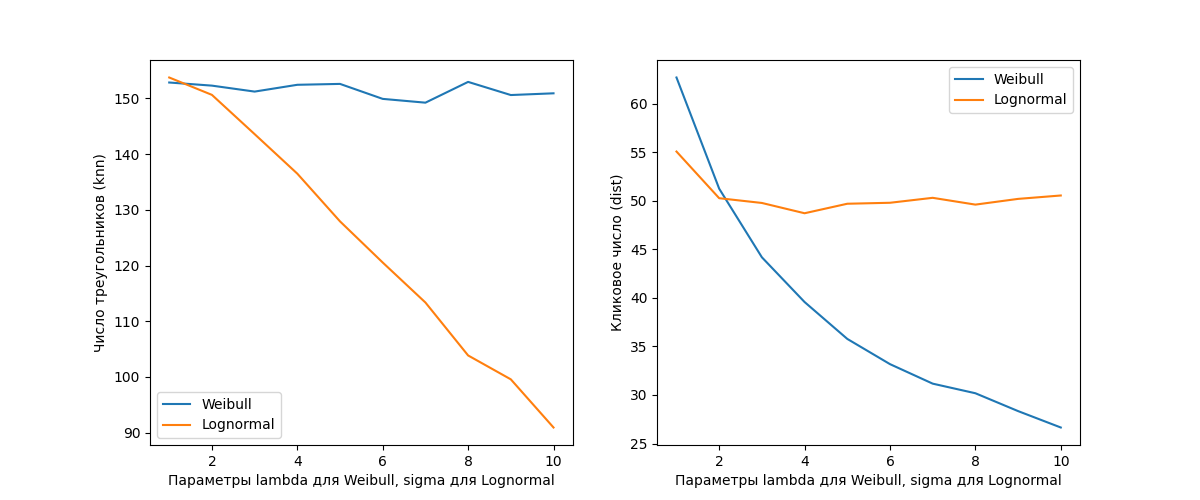
\includegraphics[width=0.95\textwidth]{Graphics/part1_results_Yaroslav.png}
    \caption{Изменение графовых метрик при варьировании параметров Weibull/Lognormal (серия Ярослава).}
    \label{fig:part1-yaroslav}
\end{figure}

\noindent\textbf{Вывод.} Метрики дистанционного графа реагируют сильнее; Lognormal приводит к более резкому разрежению графа, чем Weibull.

%--------------------------------------------------
\section*{2. Влияние параметров графа и объёма выборки (Часть\,2)}

\begin{figure}[H]
    \centering
    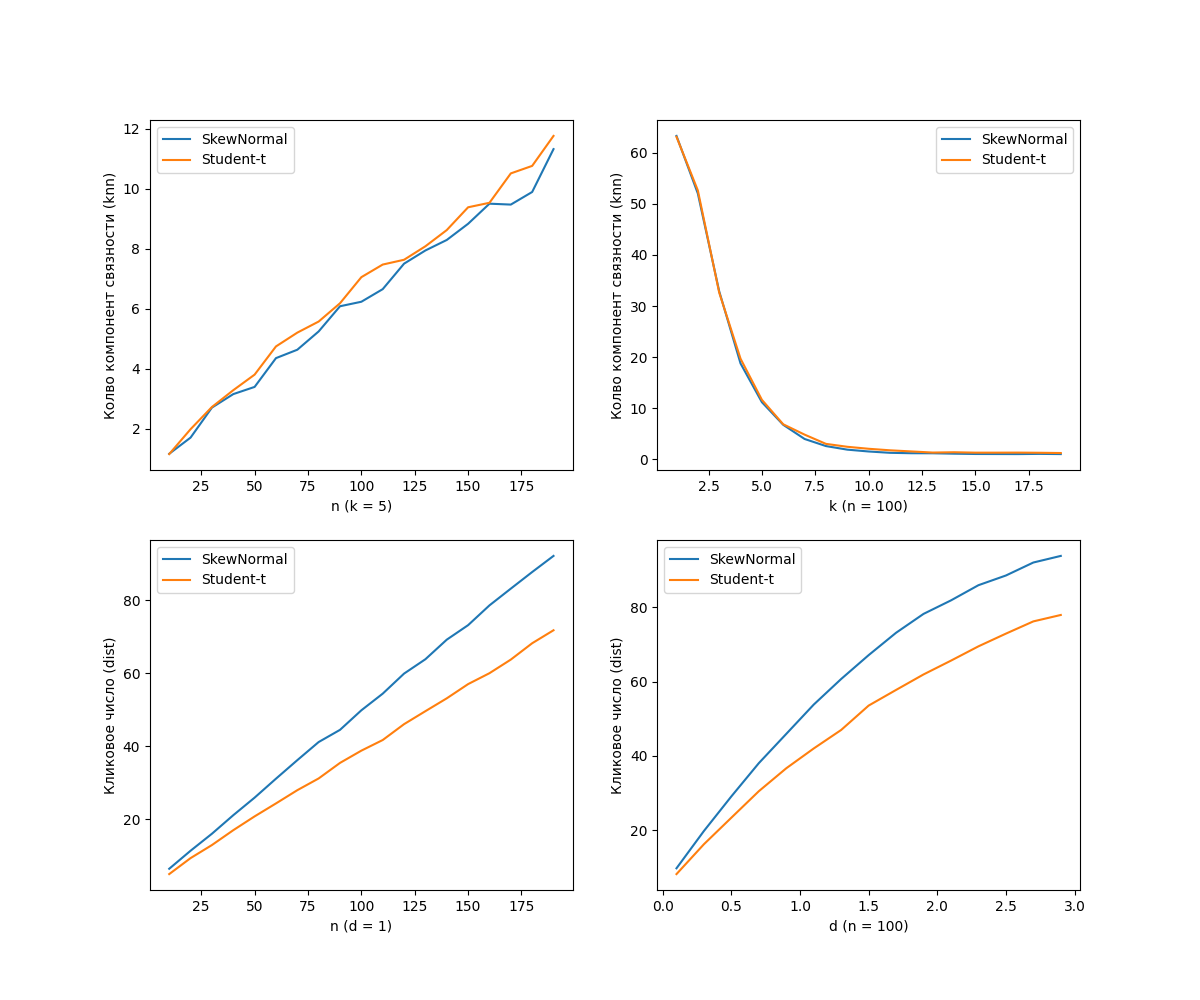
\includegraphics[width=0.95\textwidth]{Graphics/part2_results_Askar.png}
    \caption{Зависимость метрик от $n$, $k$, $d$ (серия Аскара).}
    \label{fig:part2-askar}
\end{figure}

\begin{figure}[H]
    \centering
    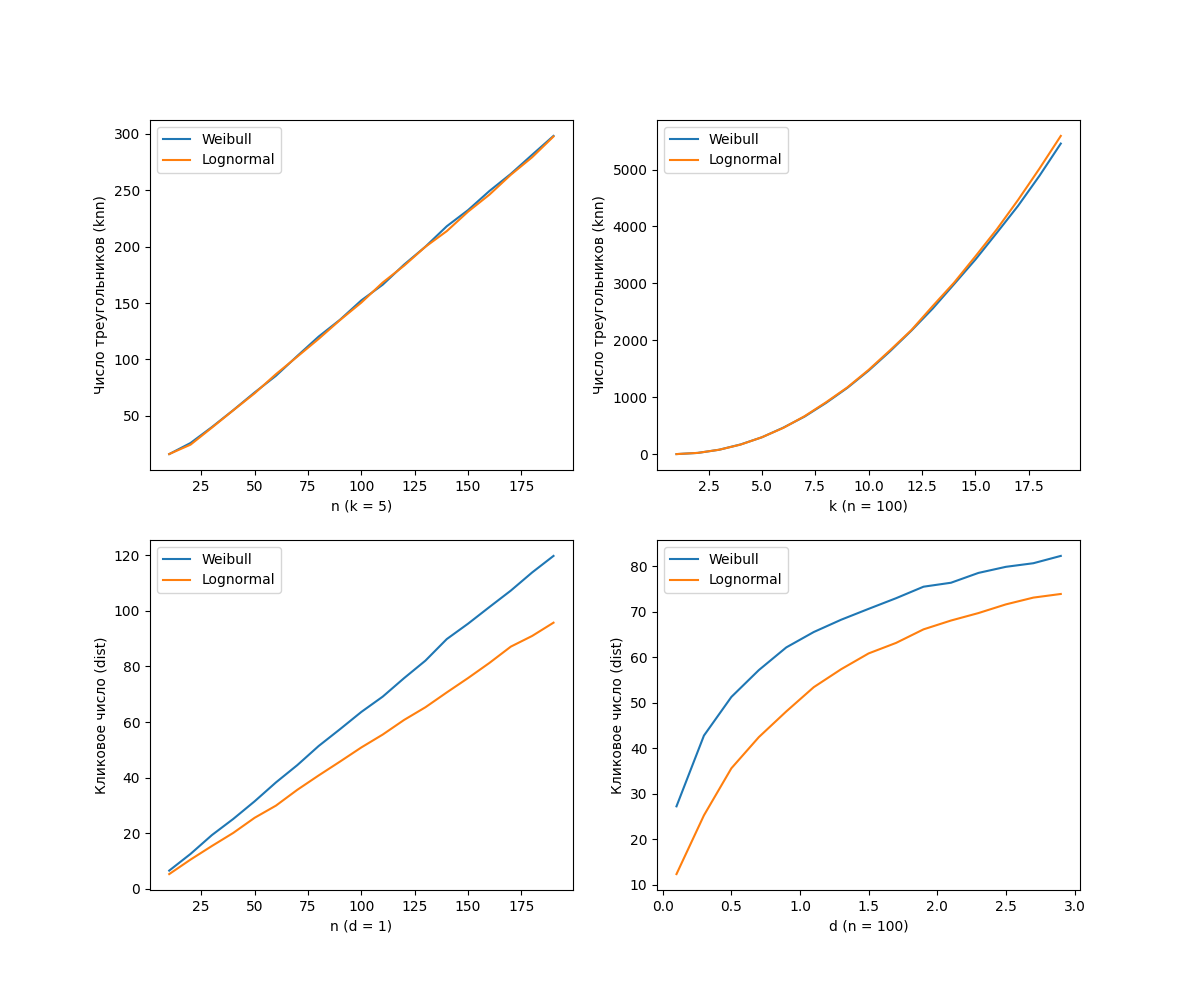
\includegraphics[width=0.95\textwidth]{Graphics/part2_results_Yaroslav.png}
    \caption{Зависимость метрик от $n$, $k$, $d$ (серия Ярослава).}
    \label{fig:part2-yaroslav}
\end{figure}

%--------------------------------------------------
\section*{3. Проверка гипотез (Часть\,3)}

\begin{figure}[H]
    \centering
    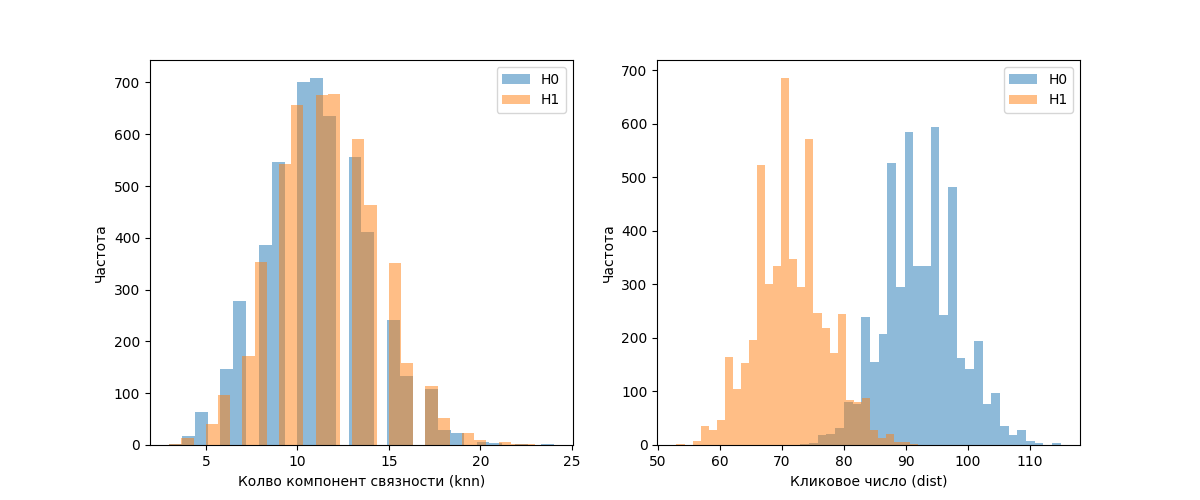
\includegraphics[width=0.95\textwidth]{Graphics/part3_results_0_Askar.png}
    \caption{Эмпирические распределения метрик под $H_0$ и $H_1$ (Askar, первый набор).}
    \label{fig:part3-0-askar}
\end{figure}

\begin{figure}[H]
    \centering
    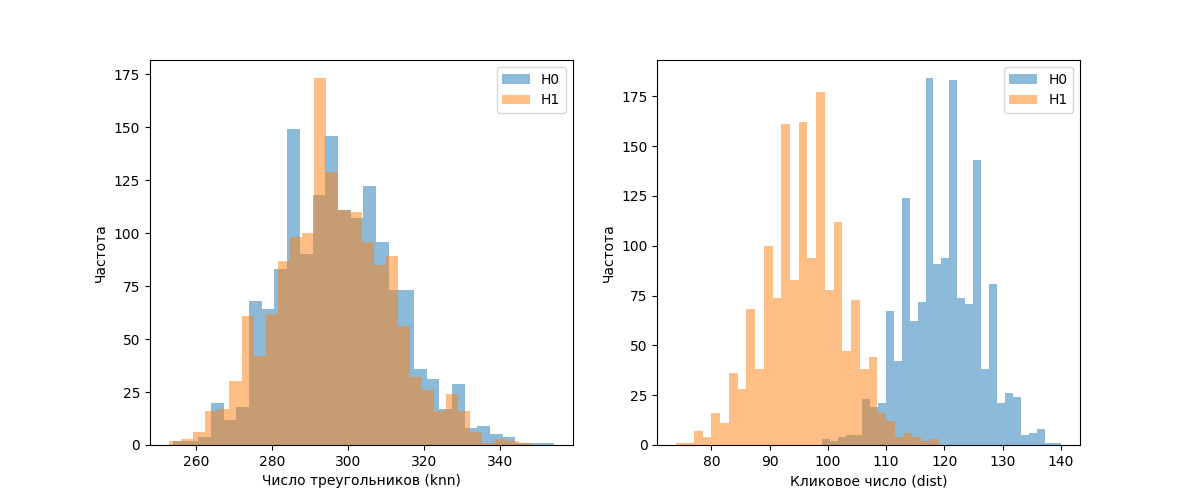
\includegraphics[width=0.95\textwidth]{Graphics/part3_results_0_Yaroslav.png}
    \caption{Эмпирические распределения метрик под $H_0$ и $H_1$ (Yaroslav, первый набор).}
    \label{fig:part3-0-yaroslav}
\end{figure}

\begin{figure}[H]
    \centering
    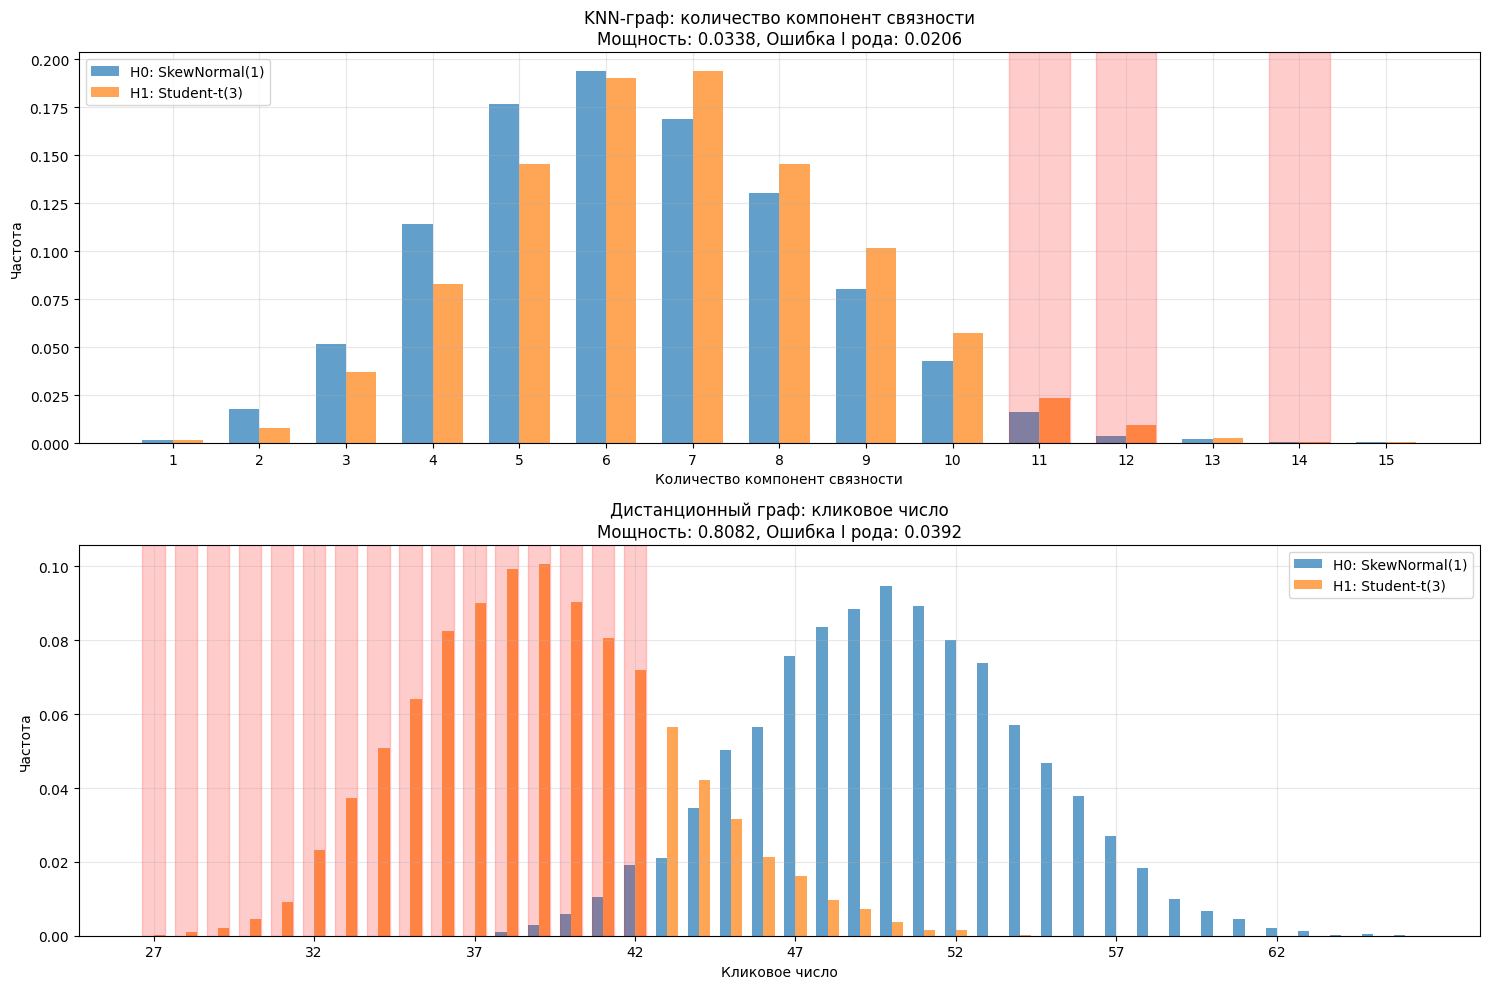
\includegraphics[width=0.95\textwidth]{Graphics/part3_results_1_Askar.png}
    \caption{Гистограммы метрик с критической областью (Askar, второй набор).}
    \label{fig:part3-1-askar}
\end{figure}

\begin{figure}[H]
    \centering
    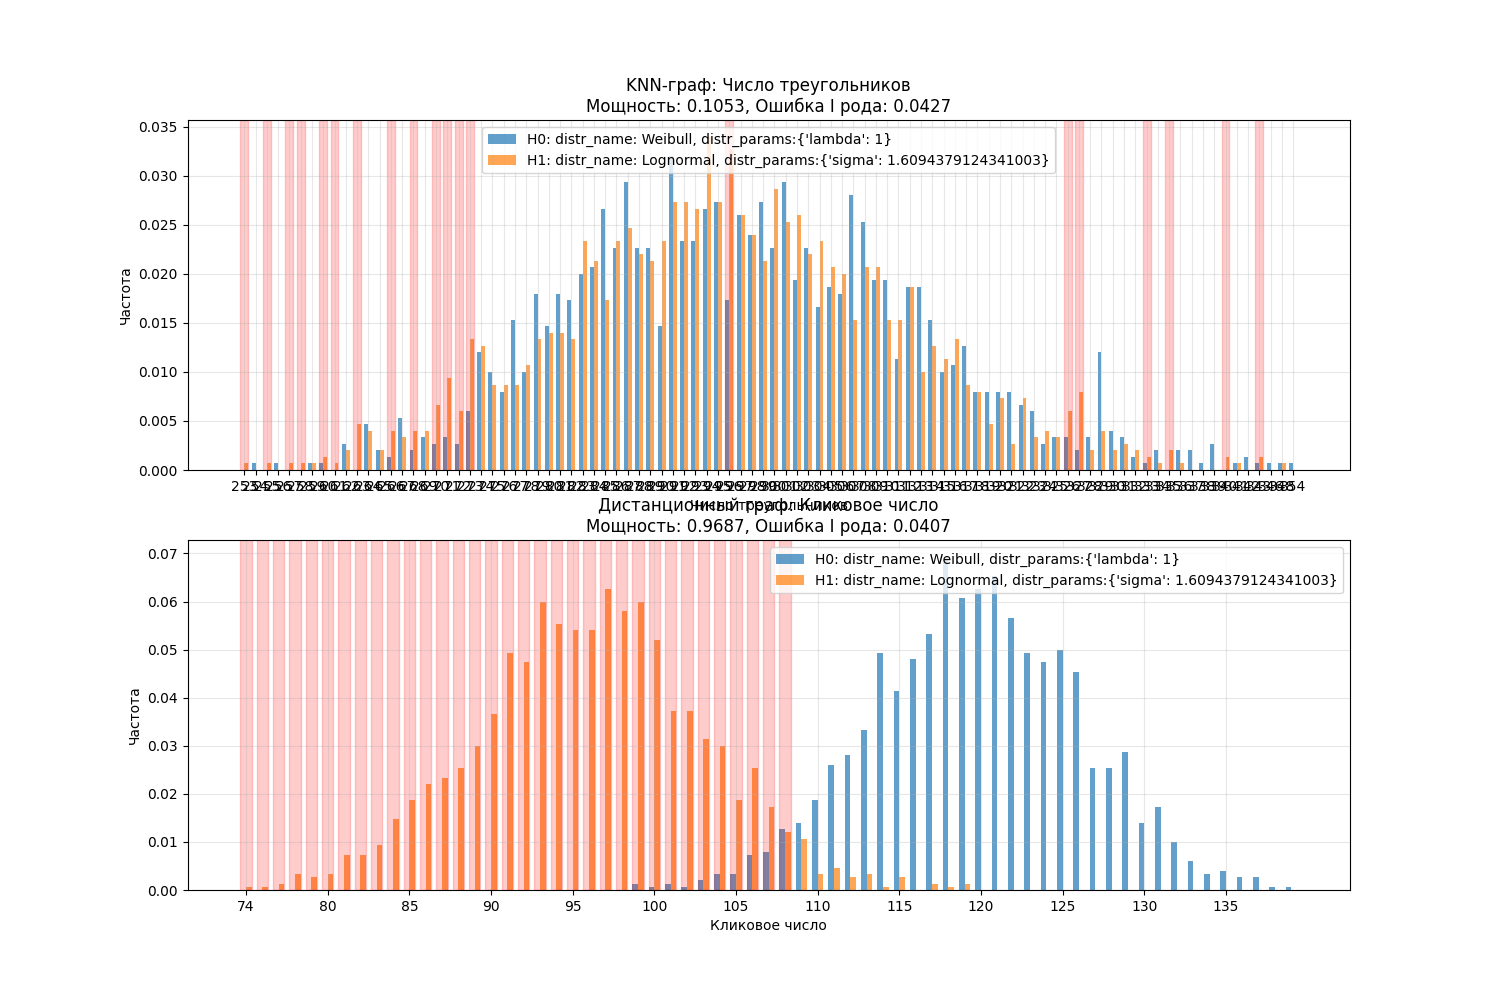
\includegraphics[width=0.95\textwidth]{Graphics/part3_results_1_Yaroslav.png}
    \caption{Гистограммы метрик с критической областью (Yaroslav, второй набор).}
    \label{fig:part3-1-yaroslav}
\end{figure}

\begin{table}[H]
    \centering
    \caption{Мощность тестов и ошибка~I рода}
    \label{tab:power}
    \begin{tabular}{@{}llll@{}}
        \toprule
        Сценарий & Метрика & Мощность $1-\beta$ & Ошибка $\alpha$ \\
        \midrule
        Askar: SkewN vs Stud-$t$ & Компоненты (k-NN) & $0.013$ & $0.007$ \\
        & Клика (dist) & $0.968$ & $0.046$ \\
        Yaroslav: Weibull vs LogN & Треугольники (k-NN) & $0.105$ & $0.043$ \\
        & Клика (dist) & $0.969$ & $0.041$ \\
        \bottomrule
    \end{tabular}
\end{table}

\noindent\textbf{Основной вывод.} Клика дистанционного графа обеспечивает наивысшую мощность (\(\approx0.97\)) при контроле уровня значимости.

%--------------------------------------------------
\section*{4. Итоговые наблюдения}

\begin{enumerate}
    \item Метрики k\nobreakdash-NN\,графа при малых $k$ мало чувствительны к различиям распределений.
    \item Дистанционный граф при подходящем пороге $d$ лучше разделяет распределения.
    \item Настройка параметров графа (особенно $d$) критична для высокой мощности статистического теста.
\end{enumerate}

\end{document}
